%auto-ignore
%      this ensures the arxiv doesn't try to start TeXing here.
%!TEX root = super_lattice_models_draft.tex
%      prev line helps TeXShop do the right thing

%%%%%%%%%%%%%%%%
\section{Kitaev chain} \label{kitaev_wire}
%%%%%%%%%%%%%%%%

In this section, we show how the graphical formalism developed in previous sections
can be used to capture the salient features of the ``Kitaev wire", 
Kitaev's toy model of a one-dimensional spinless $p$-wave superconductor \cite{kitaev2001}. 
This highlights the connection between Majorana zero modes and Ising anyons and serves 
as a nice application of the graphical calculus of the $C_2$ theory.
Most of what we say applies beyond the $C_2$ theory and can be carried out for any theory containing at least one $q$-type object.
The Hamiltonian we write down is a special case of
the one constructed in Section \ref{Super_pivotal_Hamiltonian}, for particular choices of cell decompositions of a disk (annulus) with fixed boundary conditions.
The associated wavefunctions we construct
are the same as those found in, e.g., \cite{fidkowski2011}, but presented in a more graphical formalism 
that serves as a simple example of the techniques discussed in Section \ref{state_sums}.

Recall that the $C_2$ theory has two simple objects, $\unit$ and $\beta$,
with $\beta\tp \beta\cong \cc^{1|1}\unit$,
and $\End(\beta) \cong \cliff_1$.
We will focus on the $\beta$ object in the $C_2$ 
theory for concreteness, but the analysis can be applied q-type objects $q$ in any theory.

In what follows, 
we will show that a single strand of $\beta$ string is a diagrammatic description for the zero correlation length limit of the Kitaev chain. 
This means that the string-net Hamiltonian in Section \ref{Super_pivotal_Hamiltonian} 
based on the $C_2$ theory describes a phase of fluctuating Kitaev wires, 
an idea previously investigated in \cite{tarantino2016,ware2016,kapustin2017}.

The basic strategy is to cut a single $\beta$ strand into pieces and analyze how to glue those pieces back together to recover the uncut strand. 
Physically, we will implement the gluing by requiring the vectors to be in the ground space of a particular Hamiltonian, which is similar to what we did in Section \ref{Super_pivotal_Hamiltonian}. 
We first note that the vector space associated to a single interval $I$ with boundary conditions labeled by $\beta$ can be written graphically as 
\be\label{VIbetabeta}
 A(I;\beta,\beta) = \cc \left[ \halfchain\;, \; \halfchaindot \right] \cong \cc^{1|1}.\ee
 
 Now we can consider splitting the interval $I$ into two smaller intervals $I_1,I_2$, such that $I_1\cup I_2 = I$.
 We then can reconstruct the vector space $A(I;\beta,\beta)$ from the vector 
 spaces $A(I_1;\beta,\beta),A(I_2;\beta,\beta)$ by gluing the two intervals $I_1,I_2$ together. 
Algebraically, this gluing is implemented by the tensor product. However, 
we must be sure to make the proper choice 
of tensor product to ensure that we don't produce any extra degrees of freedom during the gluing. 
The standard tensor product $\tp_\cc$ doesn't work, since then $A(I_1;\beta,\beta) \tp_\cc A(I_2;\beta,\beta) \cong \cliff_2 \not\cong A(I;\beta,\beta)$. 

The correct tensor product to use is the relative tensor product $\tp_{\End(\beta)}$ (a.k.a $\tp_{\cliff_1}$) discussed in Section \ref{modified_tensor_product}. 
With this tensor product, we (rather trivially) have 
\be A(I;\beta,\beta) \cong A(I_1;\beta,\beta) \tp_{\End(\beta)} A(I_2;\beta,\beta),\ee
which tells us how to split apart the $I$ interval correctly. 

Graphically, the relative tensor product $\tp_{\End(\beta)}$  is needed to mod out by local relations involving the sliding of fermions along $\beta$ lines, 
as was discussed Section \ref{modified_tensor_product}. 
Utilizing $\tp_{\End(\beta)}$ is equivalent to performing the regular tensor product $\tp_\cc$ and modding out by the equivalence relations
\begin{align}
\label{graphical_equiv_reln} 
\halfchain \tp_\cc \halfchaindot \; &=\; \halfchaindot \tp_\cc \halfchain\; ,\\
\nonumber
\halfchaindot \tp_{\cc} \halfchaindot \;  &= -A^4\; \halfchain \tp_{\cc}  \halfchain.
\end{align}
where we have assumed a Koszul ordering for the fermions which increases from left to right (see Table \ref{C2_data_table} for the origin of the phase $A^4$).

As we did with the string-net Hamiltonian in Section \ref{Super_pivotal_Hamiltonian}, 
we can implement these equivalence relations energetically, via an appropriately defined Hamiltonian, which 
will be the same as the edge term in the lattice Hamiltonian defined in \eqref{De_defn}. 

Consider an interval $I$ of $\beta$ string cut into $n$ segments: $I = I_1\cup I_2\cup\dots\cup I_n$.
Each segment $I_i$ will end up mapping to a single physical site in the Kitaev chain. 
The local Hilbert space at each $I_i$ segment is generated by two basis vectors $v_e,v_o$, 
which for convenience we draw as
\begin{align} \label{vevodefn}
v_e \; = \;\LocalHilba\,,\qquad v_o \; = \; \LocalHilbb\;.
\end{align}
The upward-curved ends on each $\beta$ segment are drawn purely for aesthetic purposes, and exist solely to make drawing the Kitaev chain slightly easier. 
The local Hilbert space is then
\begin{align}
A(I_i; \beta, \beta) = \cc \left[ \LocalHilba, \LocalHilbb \right] \cong \cc^{1|1}.
\end{align}


The total Hilbert space of the chain is given by tensoring each local Hilbert space together:
\begin{align} 
\label{HilbInterval}
\mch_I  = A(I_1; \beta, \beta)  \tp_\cc A(I_2; \beta, \beta)  \tp_\cc \cdots \tp_\cc A(I_n; \beta, \beta).  
\end{align} 
States in this Hilbert space are expressed graphically as
\begin{align} \label{example_hilb_vectors}
\quarterpiperprime \tp  \LocalHilba \tp  \LocalHilba \tp  &\cdots \tp  \LocalHilba \tp  \quarterpipelprime, \\
\quarterpiperdotprime \tp  \LocalHilbb \tp  \LocalHilba \tp  &\cdots \tp  \LocalHilba \tp  \quarterpipelprime, \\
\quarterpiperdotprime \tp  \LocalHilba \tp  \LocalHilbb \tp  &\cdots \tp  \LocalHilba \tp  \quarterpipelprime, \\
&\;\; \vdots
\end{align}
and so on. 
Instead of using the relative tensor product $\tp_{\End(\beta)}$ to mod out by the equivalence relations \eqref{graphical_equiv_reln} we use $\tp_\cc$ (abbreviated as $\tp$ above) and define a Hamiltonian so that the ground space is isomorphic to $A(I; \beta, \beta)$. 
The Hamiltonian can be written as:
\begin{align} \label{kitaev_chain_ham_sitei}
H_i =  \frac{1}{2} \left( \Id \;\; + \;\; \TwoLinedotdot \right),
\end{align}
which have a non-trivial action only on the adjacent Hilbert spaces associated to the intervals $I_i$ and $I_{i+1}$.%
\footnote{Note that there are no terms that act on both the right and left ends of a single strand/interval; such a term would perturb us away from the zero correlation length limit.
In the language of the Kitaev chain, this corresponds to tuning the chemical potential to zero and the 
magnitude of the superconducting gap to the hopping amplitude.}

The image of this projector on a pair of adjacent string endpoints is  
\begin{align} 
\quarterpiper \tp_\cc \quarterpipel + \quarterpiperdot \tp_\cc \quarterpipeldot\,,
\end{align}
so that using $\tp_\cc$ and projecting with $H$ is equivalent to using $\tp_{\End(\beta)}$. 
Thus, $H_i$ is responsible for gluing together ends of $\beta$ strands. 
In terms of electronic operators, $H_i$ implements hopping and pairing between electrons in nearest neighbor sites $i$ and $i+1$.

We form our Hamiltonian from a sum of projectors, $H_i$, acting between each pair of strands:
\begin{align}
\label{KWHam}
H = t \sum_{i = 1}^{n-1} (1- H_i).
\end{align}
This Hamiltonian describes the zero correlation length limit of the Kitaev chain, albeit in a slightly unconventional language.
To understand this, we proceed to investigate the ground state wave functions.

We note that the nontrivial term in the Hamiltonian is proportional to the fermion parity measured between adjacent physical sites. 
Indeed, acting with that term on the vectors $v_e,v_o$ defined in \eqref{vevodefn}, we find
\begin{align}
\TwoLinedotdot\; \circ \; v_e =\; v_e \quad \text{and} \quad \TwoLinedotdot\; \circ\; v_o \; =\;   - \; v_o.
\end{align}
which is precisely the action of $(-1)^F$ (which can be identified with $i\gamma_1\gamma_2$ in the conventional Clifford algebra language).

It is straightforward to find the ground states of \eqref{KWHam}.
Noting that the non-trivial term in the Hamiltonian is just measuring the parity shared between adjacent ``physical" sites, 
we can do a change of basis using an F-move so that the Hamiltonian is diagonal and annihilates the ground state.
In this basis the (un-normalized) ground state wavefunctions take the form
\begin{align} \label{kitaev_wire_ground_states}
\Psi_e = \;\StaggaredGSEvenprime \; \cdots \; \StaggaredGSEvenRprime\;, 
\qquad \text{and} \qquad 
\Psi_o =\; \StaggaredGSOddprime \; \cdots  \; \StaggaredGSEvenRprime\;.
\end{align}
In this basis the Hamiltonian acts as $(1-(-1)^F)$ on each pair of vertical strands, which is clearly zero.

To better understand the wavefunctions $\Psi_e,\Psi_o$, we can apply a series of F-moves to change to the physical ``on-site" basis.\footnote{Recall the physical Hilbert space is associated to $A(I_i;\beta, \beta)$, 
whereas the wavefunctions $\Psi_e,\Psi_o$ are expressed in a basis that's ``shared" between adjacent sites.}
In a Kitaev chain with $n$ physical sites (i.e., $n$ intervals), 
we recover the well known result
\begin{align}
\Psi_e = \frac{1}{d^{n-1}} \sum_{\substack{ \{ v_i\} \\  n_f = \text{even} }} (A^4)^{n_f/2} \; v_1 \tp v_2 \tp \cdots \tp v_n
\end{align}
where the sum is over all configurations of $v_i =v_o,v_e$ such that only an even number $n_f$ of odd vectors $v_o$ appear 
in the tensor product, and where $v_e,v_o$ are defined as in \eqref{vevodefn}.
For the odd wavefunction $\Psi_o$, we find 
\begin{align}
\Psi_o = \frac{1}{d^{n-1}}\sum_{\substack{ \{ v_i\} \\  n_f = \text{odd} }}  (A^4)^{(n_f-1)/2}\; v_1 \tp v_2 \tp \cdots \tp v_n
\end{align}
where the sum is now restricted so that only an odd number $n_f$ of odd vectors $v_o$ vectors in the tensor product.
From the expressions for $\Psi_e,\Psi_o$ in this basis, we see that they are given by configurations 
that are coherent sums over all fermion parity even and fermion parity odd states, respectively.  

Note that the fermion dot appearing in $\Psi_o$ of \eqref{kitaev_wire_ground_states} has zero energy (since the Hamiltonian does not act on either the beginning of the first strand in the chain or the end of the last strand), while this is not true for fermion dots 
appearing on the interior cups. 
Physically, this is due to the presence of a pair of Majorana zero modes localized at the ends of the chain. 
One can explicitly construct the zero mode operators by considering the odd operators acting on either end of the chain; 
they commute with the Hamiltonian, anti-commute with one another, anti-commute with $(-1)^{F_\text{tot}}$ (the total fermion parity), and up to a pre-factor each square to the identity.
These are exactly the properties of a Majorana zero mode. 
A nice feature of the diagrammatic notation we use is that one can easily see that acting on the left end of the chain with one zero mode operator is equivalent to acting on the right end with the other zero mode operator (up to a phase).
To see this, one simply slides the fermionic dot appearing from the zero mode operator along the bottom $\beta$ strand appearing in the presentation of the wavefunction (see \eqref{kitaev_wire_ground_states}).
Physically, this means the ends of the wire share a fermionic mode, 
and no information about the occupancy of this mode can be detected by local measurements.

By considering the same spin chain but using the regular Ising fusion category $A_3$ (rather than the condensed $A_3/\psi$ theory), one finds exactly the transverse field Ising model. 
Fermion condensation provides a map between these two models in the same way the Jordan-Wigner transformation does.
Of course, we have only discussed the zero correlation length limit, but on-site terms can be added as well, and the analysis carries through, except that the zero modes are exponentially localized to the boundary (for a small perturbation).
In the zero correlation length limit, excited states are easily constructed by putting dots on the intermediate cups. 

We now turn our attention to the Kitaev chain defined on a circle. 
The bulk of the Hamiltonian is constructed from a sum of projectors defined in \eqref{kitaev_chain_ham_sitei}. 
To ``glue" the end points of the interval into a circle, we need to add an additional term across the boundary.
There are two ways to do the gluing, differing from one another by a $2\pi$ rotation of the spin framing
(i.e.\ a spin flip). 
These choices correspond to the two spin structures on the circle, $S^1_B$ and $S^1_N$, corresponding to anti-periodic and periodic fermionic boundary conditions, respectively.
To define periodic boundary conditions we define $H_{n+1}$, the Hamiltonian term which glues the 
two endpoints of the interval together, by
\begin{align}
H_{n+1}^N = \frac{1}{2}
\left(   \; \HambdR  \cdots \HambdL \quad  +  \quad 
   \HambdLdot \cdots \HambdRdot  \;\right)    
\end{align}
where the leftmost string acts on the left side of $I_1$ and the rightmost string on the right side of $I_n$.
When closing the interval with anti-periodic boundary conditions (to form the bounding spin structure) we need to apply a spin flip twist to $H_n$, resulting in an additional minus sign multiplying the nontrivial term in the projector:
\begin{align}
H_{n+1}^B = \frac{1}{2}
\left(   \; \HambdR  \cdots \HambdL \quad  -  \quad 
   \HambdLdot \cdots \HambdRdot  \;\right)    
\end{align}
We note that these give us explicit matrices for the even linear maps $\cl_B: A(I; \beta, \beta) \to A(S^1_B, \beta)$ and $\cl_N: A(I;\beta, \beta) \to A(S^1_N,\beta)$.
In this case we are led 
to identify $\cl_B$ with $H_{n+1}^B$ and $\cl_N$ with $H_{n+1}^N$.
To substantiate these identifications we will explicitly compute the ground state wavefunctions.

In Section \ref{C2excitations} we noted that closing a q-type object along a bounding (non-bounding) spin structure results in an even (odd) parity vector; if the identifications made above are correct, then the ground state of the bounding Hamiltonian should have even parity, and the ground state of the non-bounding Hamiltonian should have odd parity. 
To see that this is indeed the case, we note that that when acting with the non-trivial term in $H^{X}_{n+1}$ for $X\in \{B,N\}$
on the the subspace spanned by \eqref{kitaev_wire_ground_states} (with the outer legs now turned up), 
we need to slide one of the fermions around the full $S^1_{X}$.
Using this, the fact that the structure of the Hamiltonian is the same as in \eqref{kitaev_chain_ham_sitei}, and using our earlier results \eqref{kitaev_wire_ground_states}, we can write the (unnormalized) wavefunctions on the $B$ and $N$ sectors as 
\begin{align} \label{kitaev_wire_circle_ground_states}
\Psi_B =  \;\StaggaredGSEven \; \cdots \; \StaggaredGSEvenR_B, 
\qquad \qquad 
\Psi_N =\; \; \StaggaredGSOdd \; \cdots  \; \StaggaredGSEvenR_N \; ,
\end{align}
where the subscripts denote the spin structure. 
Although our graphical presentation may give the impression that these pictures are drawn on an interval, they are not: the presence of the $H_{n+1}$ terms, which act on the left-most and right-most strands
in the graphical presentation of $\Psi_e$ and $\Psi_o$ are responsible for gluing the interval into a circle. 

Note that the other possible candidates for ground-state wavefunctions (an odd-parity version of $\Psi_B$ or an even-parity version of $\Psi_N$) are identically zero, which can be seen by using the graphical 
calculus of the $C_2$ theory (see the discussion around \eqref{BoundingNullVector}).

\medskip

The above Hamiltonian can be viewed as a special case of the Hamiltonian in Section \ref{Super_pivotal_Hamiltonian} as follows.
We take the ambient 2-manifold to be a long, thin rectangle (i.e.\ a disk).
We fix a $\beta$ strand boundary condition at each of the short sides of the rectangle.
On the long sides we impose empty boundary conditions.
In the interior, the ``lattice" contains only 2-valent vertices, as shown in Figure \ref{celldecompKitWire}.
Applying the general prescription in Section \ref{Super_pivotal_Hamiltonian} 
to this case yields essentially the same Kitaev wire Hamiltonian as defined above.
The spins at each 2-valent vertex are $V^{\beta\beta} \cong \cc^{1|1}$.
The vertex terms of the general Hamiltonian do nothing interesting, and there are no plaquette terms.
The edge terms of the general Hamiltonian \eqref{ham}, which we recall serve the purpose of allowing fermion dots to fluctuate along q-type strings, are the same as \eqref{kitaev_chain_ham_sitei}.
Thus, when acting on single strands of q-type string, the general Hamiltonian \eqref{ham} reduces to the Kitaev chain Hamiltonian. 

We can similarly glue the two ends of the rectangle together (either periodically or antiperiodically) to obtain
the Kitaev chain Hamiltonians for spin circles.

\begin{figure}
\centering
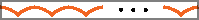
\includegraphics[scale=2.5]{celldecompKitWire.pdf}
\caption{\label{celldecompKitWire}
A cell decomposition of $I \times I$ with two marked points on the boundary, each labeled $\beta$. 
The interior graph contains $n$ ``pitchforkized" 2-valent vertices.
}
%} 
%A cell decomposition of a string-net state consisting of a single $\beta$ strand defined on $I \times I = (I\times I) \cup (I \times I) \cup (I\times I) \cup  \cdots \cup (I\times I)$.
%Each cell is given boundary conditions $\beta$ and contains one 2-valent vertex, with the vertex Hilbert space given by $A(I;\beta,\beta)$.
%The lattice Hamiltonian \eqref{ham} defined in Section \ref{Super_pivotal_Hamiltonian} has no plaquette terms in this cell decomposition and the vertex terms are trivially satisfied; hence it reduces to a sum of edge terms which are precisely equivalent to the Kitaev wire Hamiltonian \eqref{KWHam}. \ethan{sorta redundant to say this in the caption}}
\end{figure}

\medskip

We now use the Hamiltonian to construct matrix product operators (MPOs) and their related matrix product states (MPSs) for the ground state wavefunctions \eqref{kitaev_wire_ground_states} of \eqref{KWHam}.
This is a well known result, see e.g. \cite{fidkowski2011,turzillo2016,bultinck2017b}.
%\dave{Should we also cite Fidkowski-Kitaev? I think they were the first to write this down but we also cite them in the intro to the section anyway.}. 
%\ethan{sure, why not}
We write it here as it in some sense gives a ``gentler'' version of the tensor network discussed in Section \ref{state_sums}, and provides a nice application of the graphical calculus developed in the body of the paper.

We seek an MPO that projects a given state into the image of the projectors $H_i$ defined in \eqref{kitaev_chain_ham_sitei}. 
For convenience, we write $H_i =\frac{1}{2}( e_{i} + f_{i})$, with $e_{i}$ proportional to the identity operator on the junction between the intervals $I_i$ and $I_{i+1}$, and $f_{i}$ proportional to the fermion parity operator $(-1)^F$ across the junction.
Temporarily putting aside the issue of boundary conditions, to find the MPO we simply act with $\prod_i H_i$ on 
a given initial vector $V = v_1\tp \cdots \tp v_n$, where $v_i=v_e,v_o$ (graphically, these input vectors look like those appearing in \eqref{example_hilb_vectors}).
After expanding the product $\prod_i H_i$, we find an operator which is a sum over all possible configurations of the operators $e_i$ and $f_i$ straddling the junctions between intervals $I_i$ and $I_{i+1}$. 
We will denote the resulting state by $\Psi$.

We now just need to simplify the resulting state $\Psi$ using the local relations of the $C_2$ theory. 
Each physical site $v_i$ can be acted on by two terms in the Hamiltonian: $H_i$ (acting on the right strand of $v_i$) and $H_{i-1}$ (acting on the left strand). 
Hence, when we simplify $\Psi$, the phase factor associated with a given physical site $v_i$ will depend on a pair of indices $(e,e)$,$(e,f)$,$(f,e)$, and $(f,f)$, where 
the left (right) index denotes the term in $H_{i-1}$ $(H_i)$ that contributes to the phase.

Focusing on a single site with input vector $v_i$, 
we can succinctly write the action of the Hamiltonian as a matrix $(W^{v_i \to v_i'})_{xy}$, where $v_i'$ denotes the output vector obtained after acting with the Hamiltonian and where $x,y \in \{ e, f \}$.
These matrices are straightforward to compute using the rules of the $C_2$ graphical calculus.
If the input vector is $v_e$, we find
\begin{align}
W^{v_e \to v_e} = 
\frac{1}{2}\left( \begin{matrix} 
1 & 0\\
0 & 1 \\
\end{matrix} \right) \quad \quad \quad \quad 
W^{v_e \to v_o} = 
\frac{1}{2}\left( \begin{matrix} 
0& A^4\\
1 & 0 \\
\end{matrix} \right),
\end{align}
while we get
\begin{align}
W^{v_o \to v_e} = 
\frac{1}{2}\left( \begin{matrix} 
0 & 1\\
A^4 & 0\\
\end{matrix} \right) \quad \quad \quad \quad 
W^{v_o \to v_o} = 
\frac{1}{2}\left( \begin{matrix} 
1& 0\\
0 & -1 \\
\end{matrix} \right)
\end{align}
if the initial input vector is $v_o$.

We thus obtain an MPO on the interval:
\begin{align}
W_{b_l b_r}: \; \mch_I &\to \mch_I\\
v_1 \tp \cdots \tp v_n& \mapsto  \sum_{\{v_i' \}} \left( W^{v_1 \ra v_1'} W^{v_2 \ra v_2'} \cdots W^{v_n \ra v_n'} \right)_{b_l b_r} \; v_1' \tp \cdots \tp v_n' ,
\end{align}
where $b_l,b_r \in \{e,f\}$ and $b_r$ are boundary conditions for the interval.
If $b_l=f$ ($b_r=f$), an additional fermionic dot is present on the left side of the first interval (right side of the last interval). 
For example, the diagrammatics allows one to check that $W_{ef}$ is an odd operator which satisfies $W_{ef} = A^4 W_{fe} \circ (-1)^F$.This is a consequence of $\beta$ having an odd endomorphism.
The additional $(-1)^F$ accounts for sliding a fermion past an odd operator.

To obtain an MPS for the ground states, we simply fix an initial vector $v_1\tp \dots \tp v_n$ and boundary conditions for the MPO. 
On the interval we can construct the even parity ground state by
\begin{align}
\Psi_{e} = \sum_{\{v_i' \}} \left( W^{v_e \ra v_1'} W^{v_e \ra v_2'} \cdots W^{v_e \ra v_n'} \right)_{ee} \; v_1' \tp \cdots \tp v_n' 
\end{align} 
and the odd parity ground state with
\begin{align}
\Psi_{o} = \sum_{\{v_i' \}} \left( W^{v_o \ra v_1'} W^{v_e \ra v_2'} \cdots W^{v_e \ra v_n'} \right)_{ee} \; v_1' \tp \cdots \tp v_n'.
\end{align} 
Setting the boundary conditions to be $b_l=b_r=f$ in both cases would provide the same wavefunction up to an overall phase.

Similarly using \eqref{bounding_trace}, one can find the (unnormalized) MPS on a bounding spin circle by
\begin{align} 
\Psi_B = \sum_{\{ v_i ' \} } \tr \left( W^{v_e \ra v_1'} W^{v_e \ra v_2'} \cdots W^{v_e \ra v_n'} \right) v_1' \tp \cdots \tp v_n' 
\end{align}
and by using \eqref{nonbounding_trace} we find the (unnormalized) MPS on the non-bounding circle:
\begin{align} 
\Psi_N = \sum_{\{ v_i ' \} } \str \left( W^{v_o \ra v_1'} W^{v_e \ra v_2'} \cdots W^{v_e \ra v_n'} \right) v_1' \tp \cdots \tp v_n'.
\end{align}
In order to produce a non-zero state we need to choose a even parity initial vector for the bounding spin structure, 
and an odd parity initial vector for the non-bounding spin structure. 

\begin{comment}

\dave{I think the next two paragraphs can be removed now.}
%Explicilty, in terms of basis vectors we have,
%\begin{align}
%v_1 \tp \cdots \tp v_n \xrightarrow{\quad A_{b_l b_r} \quad }
 %\sum_{\{v_i' \}} \left( A^{v_1 \ra v_1'} A^{v_2 \ra v_2'} \cdots A^{v_n \ra v_n'} \right)_{b_l b_r} \; v_1' \tp \cdots \tp v_n' 
%\end{align}


We thus obtain the MPO
\be
A = \sum_{\{ v_{i} \} , \{v_i'\}} \cdots A^{v_i \to v_i' } A^{v_{i+1} \to v_{i+1}'} \cdots,
\ee
which is a linear map from $\mch_I \to \mch_I$.

\dave{Need to do boundary conditions a little more carefully.}
\ethan{not sure wether we wanted braket notation here or not}
\dave{Yea, it's annoying. 
I was thinking we could do something like $\Psi = \sum_{...} (A^{v_1 \to v_1'} \cdots A^{v_n \to v_n'})_{v_l v_r} v_1' \tp \cdots c_n'$.} 
To obtain an MPS, we simply need to choose an input vector $V = v_1\tp \dots \tp v_n$.
The simplest choice is to fix the labels of one side of the MPO to be $V_e = v_e ^{\tp n}$ for the even parity state, and $V_o = v_o \tp v_e^{\tp (n-1)}$ for the odd parity state.
%The simplest choice is to build the MPS over the vacuum, by setting $V = v_e^{\tp N}$. 
With this, we can write the MPS on an interval as 
\begin{align} \Psi_{I,e} = \sum_{v'_i = v_e,v_o}\langle b_L | A^{v_e\ra v'_1} \cdots A^{v_e\ra v'_N} | b_R\rangle v'_1\tp \dots \tp v'_N,\end{align}
for the even parity state, and 
\be \Psi_{I,o} = \sum_{v'_i = v_e,v_o}\langle b_L | A^{v_o\ra v'_1}A^{v_e\ra v'_2} \cdots A^{v_e\ra v'_N} | b_R\rangle v'_1\tp \dots \tp v'_N,\ee
for the odd parity state. 
In the above equations, $|b_L\rangle$ and $|b_R\rangle$ denote a choice of boundary conditions on the left and right ends of the interval, respectively. 

For an MPS defined on a circle, we can use our earlier results \eqref{bounding_trace} and \eqref{nonbounding_trace} on 
partition functions to obtain 
\be \Psi_B = \sum_{ v'_i =v_e,v_o }\tr(A^{v_e\ra v'_1} \cdots A^{v_e\ra v'_N}) v'_1 \tp \cdots \tp v'_N \ee
if we are working on the bounding spin circle $S^1_B$, and 
\dave{Needs an odd endomorphism.}
\ethan{?}
\ethan{ah, I think I see what you mean. How is it now?}
\dave{Mhmm. I think so but need to double check. 
I re-did some notation and copied these paragraphs above.}
\begin{align}
 \Psi_N & = \sum_{v'_i =v_e,v_o  }\tr((-1)^FA^{v_o\ra v'_1}A^{v_e\ra v'_2} \cdots A^{v_e\ra v'_N}) v'_1 \tp \cdots \tp v'_n \\ 
 & =\sum_{v'_i =v_e,v_o }\str(A^{v_o\ra v'_1} A^{v_e\ra v'_2}\cdots A^{v_e\ra v'_N}) v'_1 \tp \cdots \tp v'_n
 \end{align}
if we are working on the non-bounding circle $S^1_N$. 

%\ethan{is the following paragraph needed anymore?}
%\dave{Don't think so.}
%\dave{Perhaps say it's actually an MPO, need to talk about gluing interval into circle. 
%Anything else?}
%MPO is:
%\begin{align}
%A = \sum_{\{ v_{i} \} , \{v_i'\}} \cdots A^{v_i \to v_i' } A^{v_{i+1} \to v_{i+1}'} \cdots
%\end{align}

%\ethan{Dave might have to change notation to find something he's happy with}
%\dave{I think we need to specify the matrices $A^{v_i}$ if we want to keep this paragraph (and I do think it's a good idea to keep).
%Also need to change to the notation we used in the rest of this section, i.e., no partition function discussion, $a_i$ no longer around, etc.}
%\dave{Anything we want to shuffle from this paragraph to the one above?}
%\dave{
%I can do this paragraph, probably this afternoon.
%Will say something like: If Hamiltonain $H_i= e_{i+1/2} + z_{i+1/2}$ then we can write the GSWF as $\psi = \sum_{\{ v_i \}}\tr (A^{v_1} \cdots A^{v_n}) $. 
%Where $A^{v_i}$ is a 2 by 2 matrix with elements 
%$(A^{v_i})_{e_{i-1/2} e_{i+1/2}}$, 
%$(A^{v_i})_{e_{i-1/2} z_{i+1/2}}$, 
%$(A^{v_i})_{z_{i-1/2} e_{i+1/2}}$, 
%$(A^{v_i})_{z_{i-1/2} z_{i+1/2}}$.
%The matrix elements are determined by the linear relations of the $C_2$ theory. }
%Note that the way we draw vectors in the Hilbert space of the Kitaev wire is essentially a graphical presentation of a matrix product state (MPS)
%\dave{I don't think I agree.
%But also not sure what you meant, see the re-write above and let me know if it makes sense.}. 
%In the MPS formalism, a site $i$ labeled by the basis vector $a_i$ is attached 
%to is associated with a matrix $A^{a_i}_{xy}$, where $x,y$ are virtual indices. 
%The $A^{a_i}$ matrices can be determined from the shadow world approach, and in this case are given by the structure constants of $\cliff_1$ \cite{turzillo2016}. 
%Wavefunctions are then constructed by contracting the virtual indices following the 
%shadow world prescription. To construct a wavefunction $|\Psi\rangle$ we need to compute 
%partition functions of the form $Z(M;\emptyset,v_1)$, where $\emptyset$ denotes 
%the input vacuum state. 
%By using our earlier results \eqref{bounding_trace} and \eqref{nonbounding_trace} on 
%partition functions, we see that 
%\dave{I don't understand how this is compatible with \eqref{graphical_MPS_state} and \eqref{kitaev_wire_circle_ground_states}. 
%It seems like \eqref{kitaev_wire_circle_ground_states} requires all $a_i = \beta$. }
%\be |\Psi\rangle = \sum_{\{ a_i \} }\tr(A^{a_1} \cdots A^{a_N}) \ket{a_1 \cdots a_n} \ee
%if the Kitaev wire is defined over an interval or on $S^1_B$, and 
%\begin{align}
 %|\Psi\rangle & = \sum_{\{ a_i \} }\tr((-1)^FA^{a_1} \cdots A^{a_N}) \ket{a_1 \cdots a_n} \\ 
% & =\sum_{\{ a_i \} }\str(A^{a_1} \cdots A^{a_N}) \ket{a_1 \cdots a_n} 
% \end{align}
%if the wire is defined on $S^1_N$. 
%This is the presentation of the wavefunctions used in the tensor network community, 
%and agrees with the results of \cite{turzillo2016,bultinck2017b}. 
%The graphical depiction of these states is given by the $\Psi_B,\Psi_N$ appearing in \eqref{kitaev_wire_circle_ground_states}. 

\end{comment}


To summarize, we showed that strands of q-type objects are intimately related to the Kitaev chain. 
One can think of the string net Hamiltonian (defined in Section~\ref{def_sect}) for the $C_2$ theory as describing a phase of fluctuating Kitaev wires, a point of view adopted in \cite{tarantino2016,ware2016,kapustin2017}.
We also noted that fermion condensation is closely tied with the Jordan-Wigner transformation, as one 
With the one-dimensional Hamiltonian at hand, we showed how to explicitly construct the MPS for the ground state wavefunctions in this graphical language, recovering the same MPS as \cite{fidkowski2011,turzillo2016,bultinck2017b}.
\begin{comment} 
%\ethan{I still don't see how these are the same MPS. %Our matrices are different (we have $A^4$s), and our hilbert space is also different %(their physical index runs over $\unit,\beta$, while we treat the odd and even parts %of $\beta$ separately).}
%\dave{Can you refer to an exact equation? 
%I think I found one of the references was using the same matrices up to a gauge transformation, but I forget which ref and where (you can always send $A_i \tp U_i^{\dagger} A_i U_{i+1}$).
%}
%\ethan{actually, I think this is just me being a bit thick and just not understanding the point of this approach to MPS, but I see it now. I retract my earlier objection} 
\ethan{something like:}
We also note that the same MPS can be found by employing the shadow world construction outlined in Section~\ref{shadowworld}. We work on the 3-manifold $D\times I$ where $D$ is a disk,  
and fix the string-net graph $w$ on the $D \times \{1\}$ boundary to have two marked $\beta$ points on the disk boundary and $n$ interior 2-valent vertices. 
When the Hamiltonian defined in Section \ref{Super_pivotal_Hamiltonian} acts on the state prepared in this way by the shadow world, the vertex and plaquette terms are trivially satisfied, 
and the edge term is identical to the Kitaev wire Hamiltonian. \dave{Should we say the plaquette term is trivially satisfied or not present?}
\kw{I prefer not present}
\end{comment}

\medskip

We also note that the same MPS can be found by employing the shadow world construction outlined in Section~\ref{shadowworld}: we work on the 3-manifold $D\times I$ where $D$ is a disk,  
and fix the string-net graph $w$ on the $D \times \{1\}$ boundary to have two marked $\beta$ points on the disk boundary and $n$ interior 2-valent vertices (this string-net state is illustrated in Figure \ref{celldecompKitWire}, where $w$ is illustrated as being made up of a union of intervals).

%\kw{We can probably delete this paragraph and instead use the one I inserted before 
%the MPS discussion; also could take material from here and add it to the other paragraph}
%\ethan{grabbed some material; I think it can be deleted now.}
%\dave{I think we can drop this paragraph, looks like the content is roughly the same.}
%Finally, we should point out that the Kitaev Hamiltonian constructed in this section is just a special 
%case of the lattice Hamiltonian defined in Section \ref{Super_pivotal_Hamiltonian}.
%Consider a cell decomposition of a single $\beta$ strand defined on $I\times I$, which is illustrated in Figure \ref{celldecompKitWire}. 
%When we consider the action of the lattice Hamiltonian in Section \ref{Super_pivotal_Hamiltonian} on this state, we see that 
%the vertex terms are trivially satisfied and the plaquette terms are absent, leaving only the edge terms. 
%These edge terms, which we recall serve the purpose of allowing fermion dots to fluctuate along q-type strings, act on this state in
%exactly the same way as the projectors constructed in \eqref{kitaev_chain_ham_sitei}.  
%Thus, when acting on single strands of q-type string, the lattice Hamiltonian \eqref{ham} reduces to the Kitaev chain Hamiltonian. 


